\documentclass[letterpaper, 10pt]{article}
\usepackage{amsmath, bbm}
\usepackage{amssymb, amsthm}
%\usepackage{mathptmx}
%\usepackage[LY1]{fontenc}
\usepackage{fancyhdr}
\usepackage{graphicx}
\usepackage{subfigure}
\usepackage{verbatim}
\usepackage{array}
\usepackage{hyperref}
\usepackage[squaren]{SIunits}
\usepackage{color}

\topmargin 0in
\headheight 0.0pt

\headsep 0. in
%\bottommargin 1in
\oddsidemargin 0.0 in
\evensidemargin 0.0 in
\textwidth 6.5 in
\textheight 9 in

\renewcommand{\headrulewidth}{0pt}
\newcommand{\tmop}[1]{\operatorname{#1}}
\newtheorem{lemma}{Lemma}
\newtheorem{theorem}{Theorem}
\newtheorem{definition}{Definition}
\newtheorem{claim}{Claim}
\newtheorem{proposition}{Proposition}


\newcommand{\neal}[1]{\textcolor{red}{Neal: #1}}
\newtheorem{corollary}{Corollary}
\newtheorem{fact}{Fact}
%%%%%%%%%%%%%%%%%%%%%%%%%%%%%%%%%%%%%%
%%       EDIT THESE VARAIBLES       %%
%%%%%%%%%%%%%%%%%%%%%%%%%%%%%%%%%%%%%%


%%%%%%%%%%%%%%%%%%%%%%%%%%%%%%%%%%%%%
%%%%%%%%%%%%%%%%%%%%%%%%%%%%%%%%%%%%%%
    \newcommand\independent{\protect\mathpalette{\protect\independenT}{\perp}}
    \def\independenT#1#2{\mathrel{\setbox0\hbox{$#1#2$}%
    \copy0\kern-\wd0\mkern4mu\box0}} 
    \numberwithin{equation}{section} 
\author{Neal Wadhwa}
\title{Phase Model for Motion Dynamic Range Compression}
\date{January 28, 2014}
\begin{document}
\newcommand{\D}{\mathcal{D}}
\newcommand{\pr}{\tmop{Pr}}
\newcommand{\R}{\mathbb{R}}
\newcommand{\beq}{\begin{equation}}
\newcommand{\eeq}{\end{equation}}
\newcommand{\E}{\mathbb{E}}
\newcommand{\Var}{\text{Var}}
\noindent
\maketitle
\section{Introduction and Background}
In this project, our ultimate goal is to take a video as an input and amplify all small motions in the scene without amplifying the noise. We can model the noiseless video as following the dead-leaves model with each ``leaf'' vibrating with a narrowband temporal motion signal. I think that there are two different types of noise in the input video that end up producing noise in the phase signal: IID additive Gaussian white noise ({\em Image Noise}) to the pixel intensity values. In the phase domain, image noise results in approximately Gaussian noise that has variance inversely proportional the amplitude of the CSP coefficients while motion noise results in additive Gaussian noise. The noise at a pixel is correlated with pixels nearby in space, but not in time. 

Because both noises are approximately Gaussian in the phase domain, linear filtering techniques are optimal and we can compute the optimal linear filter using by minimizing MMSE. The primarily challenge lies in the fact that noise is not stationary in space, due to the fact that the phase signal is stronger at edges rather than textureless regions. However, if we assume stationarity in time (i.e. a mostly static video), we can use optimal linearMMSE filtering in time to denoise the phase signal. We use a variant of Weiner Filtering, that does not depend on knowing the signal statistics. Specifically, we minimize the error between a time shifted version of the phase signal and the filtered phase signal. This removes broadband signals, such as IID Gaussian noise, while preserving narrowband signals as the latter is correlated with time-shifted versions of itself. We make the assumption that the video is mostly static, so we can assume stationarity in time.

This automatic filtering seems to produce slightly better results than just highpassing the phase signal and the noise framework is promising. The main challenge will be to figure out how to handle the nonstationarity of the noise to allow for spatial filtering and online filtering. As an ad-hoc solution for now, we use an amplitude squared weighted blur to spatially denoise the phases and provide some justification for it. 

In the future, we can change the signal model to be less restrictive than the dead leaves model and instead include spatial coherence. We can also try to handle the nonstationarity of the amplitude signal and do optimal linear MMSE filtering in space and in time. 



%Because the motions will occur over several frames and will generally be represented as a time series at every pixel, we seek to compress the range of motion energies (over a short time window) rather than the exact motions at any given time. Therefore, our goal is to estimate the spatially-varying denoised motion energy and then use this to produce a spatially varying amplification factor over the video. 

%We compute the motion using the local phase in spatially bandpassed versions of the image. To get a sense of how to denoise the phase and compute the motion energy, without adding noise energy, we propose a simple model of the phase and amplitude signal and noise in these spatially bandpassed videos and then find an optimal estimate of the motion energy. We demonstrate how good our noise model on the phases is using synthetic data and then compute the optimal estimator of the motion energy. 





\section{Forward Model}
We give a forward model for the phase signal in this section. For a given amplitude and phase, there are two sources of noise, image noise and motion noise. We assume that the first follows a distribution that is dependent on the amplitude to image noise ratio. For low values, it is uniform and for high values it is Gaussian. We assume the motion noise is independent of the amplitude and manifests as Gaussian noise. In reality, this second noise models the fact that the displacement is related to the phase variations to a first order through the instaneous frequency, but the instataneous frequency is only approximately constant as the bandwidth of the bandpass filters is not zero. 

As for signal, we assume it is narrowband and for now don't make any spatial assumptions, though in the future we would like to integrate spatial coherence into this model. The observed variables are given by 
\beq O_{x,y,t} = P_{x,y,t}+N_I + N_M \eeq
%and we want to estimate the motion energy (as represented by the phases)
%\beq \sqrt{\sum_t P_{x,y,t}^2 } \label{eq:goal}\eeq
%It would be sufficient to estimate $P_{x,y,t}$, but we may be able to do better by just estimating the quantity in Eq.~\ref{eq:goal}. 

%We do this by first giving a forward model of a video and then doing our phase processing on it. We could try performing inference on the original video, but this would involve solving motion estimation, which is a difficult problem. So, we will just do inference on the phases in an attempt to infer a denoised phase signal. 

%We model the video as a static image with components that oscillate. The static image is four Gaussian blurred disks equally spaced apart in the image. Each disk oscillates in time with a sinusoidal motion. The frequency and amplitude are generated from  a $\frac{1}{x^2}$ distribution. The phase is chosen uniformly at random and the $x$ and $y$ components of the motion are drawn independently. This process gives a distribution $P$ from which to draw a video $I(x,y,t)$ at random. Spatiotemporal Gaussian noise is added to the image and the motion signal. 

\begin{figure}
\begin{tabular}{cccc}
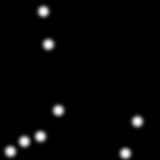
\includegraphics[width=0.23\textwidth]{figsPhaseModel01/amp.png}&
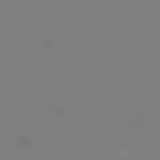
\includegraphics[width=0.23\textwidth]{figsPhaseModel01/phaseSig_m0_i0.png}&
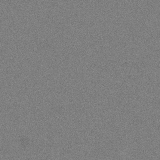
\includegraphics[width=0.23\textwidth]{figsPhaseModel01/phaseSig_m1_i0.png}&
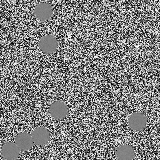
\includegraphics[width=0.23\textwidth]{figsPhaseModel01/phaseSig_m1_i1.png}\\
(a) Sample amplitude & (b) Phase Signal  & (c) With motion noise & (d) With both noises\\
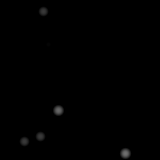
\includegraphics[width=0.23\textwidth]{figsPhaseModel01/energy_m0_i0.png}&
\setlength\fboxsep{0pt}
\fbox{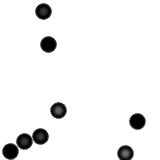
\includegraphics[width=0.23\textwidth]{figsPhaseModel01/energy_m0_i1.png}} &
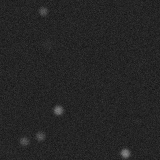
\includegraphics[width=0.23\textwidth]{figsPhaseModel01/energy_m1_i0.png}&
\setlength\fboxsep{0pt}
\fbox{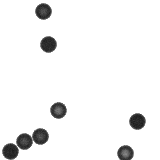
\includegraphics[width=0.23\textwidth]{figsPhaseModel01/energy_m1_i1.png}}\\
(d) Motion Energy  & (e) With image noise  & (f) With motion noise & (g) With both\\
\end{tabular}
\caption{A sample drawn from our forward model. The amplitude (a), clean phase (b), phase with motion noise (c) and phase with both types of noise (d) are shown. In addition, the temporal energy of the clean signal (e) and noisy signal (e-g), with both types of noise are shown (g). }
\end{figure}

%Once the video is generated, the amplitude and phase signal are computed using any pyramid of interest. For now, we can use either the Riesz pyramid or a four orientation, complex steerable pyramid. We can use $P$ plus our knowledge of what the various pyramids do to get a probabillity distribution on the phase, (orientation in the case of the Riesz pyramid) and amplitudes generated by the pyramid. And we can use this to infer the motion energy, without adding the noise energy. 

%The noise in the motion signal may give us regions in which the phase signal is spatially incoherent. We would hope that if the SNR is too low, our estimated motion energy is zero at such locations. In a future model, we might replace the four disks with a dead leaves model to handle occlusion and multiple motions at the same point. 


\section{Estimators}
\subsection{Motion Noise}
%First, we start with the optimal Weiner estimator. Since we are modelling the motion noise as Gaussian IID noise, the optimal linear estimator in the MMSE sense is simply
%\beq \hat I(\vec \omega) = I(\vec \omega) \frac{S_s(\vec \omega) }{S_s(\vec \omega) +S_n(\vec \omega) } \eeq
%where $\vec \omega$ is a vector representing the frequency in space and time. This produces reasonable results (Fig.~\ref{fig:weinerMotionNoise}). Because we know the exact generative model of the signal and noise, we can estimate their spectra using monte carlo simulation (Fig.~\ref{fig:weinerMotionNoise}).



\paragraph{Motion Noise is Gaussian Assumption}  See Fig.~\ref{fig:motionNoise}.
\begin{figure}
\begin{tabular}{cccc}
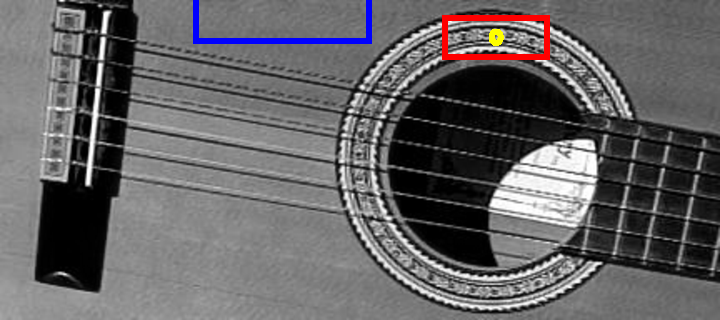
\includegraphics[width=0.2\textwidth]{motionNoiseGaussian/guitar.pdf} &
\includegraphics[width=0.2\textwidth]{motionNoiseGaussian/imageNoiseHistogram.eps} &
\includegraphics[width=0.2\textwidth]{motionNoiseGaussian/motionNoiseHistogram.eps} &
\includegraphics[width=0.2\textwidth]{motionNoiseGaussian/crossCorrelation.eps} \\
(a) Frame from Video & (b) Intensity Noise & (c) Motion Noise & (d) Cross correlation\\
\end{tabular}
\caption{We demonstrate that on a real video of a guitar (a) that the noise in intensities (b) and motion noise (c) are approximately Gaussian. The intensity noise ($\sigma = 0.02$) was computed by assuming that the region in blue was spatially constant. Once computed, the regions of high amplitude to noise ratios (>100), such as the one in red were chosen to estimate the motion noise (c, $\sigma=0.02$). This provides some evidence that our model is reasonable. However, the auto correlation shows some correlations, especially in the low frequencies. If this is noise, it shows a problem in our model}
\label{fig:motionNoise}
\end{figure}

\subsection{Image Noise}
To analyze the non stationary image noise, we consider the problem of estimating the mean of Gaussian-distributed random variables with the same mean and known, but varying variances from a weighted average of the random variables. For random variables $X_i$ with variances $\frac{\sigma^2}{A_i^2}$, their weighted average $\frac{\sum_i w_iX_i}{\sum_i w_i}$ has variance
\beq  V_w = \frac{\sigma^2}{(\sum_i w_i)^2} \left(\sum_i\frac{w_i^2}{A_i^2}\right)\eeq
We can use differential calculs to compute the partial derivatives
\beq \frac{\partial V_w}{\partial w_j} = \frac{\sigma^2}{(\sum_i w_i)^3}\left(\sum_i \frac{2 w_i w_j}{A_j^2}-2\frac{w_i^2}{A_i^2}\right)\eeq
A zero of this system and a stationary point of the variance as a function of the weights is $w_i = A_i^2$. For two variables, it is easy to show that this is a local minima. For large amplitudes $A$, image noise can be approximated by Gaussian noise with variance proportional $\frac{1}{A^2}$. As a result, we propose that any weighted average of the image noise be weighted by the square of the amplitudes. This is different than what we did in our SIGGRAPH paper.  

\paragraph{Image Noise is Gaussian Assumption}
The phase signal is a wrapped quantity with a range from $[-\pi,\pi]$. This means that it cannot be modelled by Gaussian noise. However, we show in this section that Gaussian noise is a good approximation to what the noise actually looks like. In a previous document, we showed that the phase signal has distribution 
\beq \mathcal{P}_{A_0,\theta_0}(\theta) = \frac{1}{2\pi} \text{exp}\left[-\frac{\beta^2\sin^2(\theta-\theta_0)}{2} \right]\left(\text{exp}\left[-\frac{\beta^2\cos^2(\theta-\theta_0)}{2}\right]+\beta\cos(\theta-\theta_0)\sqrt{\frac{\pi}{2}}\left(1+\text{erf}\left(\frac{\beta\cos(\theta-\theta_0)}{\sqrt{2}} \right)\right)\right) \label{eq:noisePDF01}\eeq
where $\beta$ is the amplitude to noise ratio. If we make the assumption that $\beta >>1$, that is the amplitude is much larger than the image noise, we can approximate Eq.~\ref{eq:noisePDF01} as
\beq \frac{\beta}{\sqrt{2\pi}} e^{-\frac{\beta^2(\theta-\theta_0)^2}{2}}\eeq
which is Gaussian. This breaks down when $\beta<<1$. By assuming the noise is Gaussian, we will overestimate the variance and downweight low amplitude points more than we should. However, I doubt this will make a huge difference as these points are typically so unreliable that they are already downweighted substantially.


\subsection{No Large Motion Assumption}
We assume that there are no large motions, so that both the image and motion noises are stationary in time. This allows us to perform Weiner filtering on the phase variation signal for each point. Traditional Weiner filtering requires that we know the second order statistics of the signal and noise. Since we do not really know these things, instead we make the assumption that the signal $d[n]$ is narrowband, while the noise $v[n]$ is broadband. and that the noise is decorrlated in time for lags greater than $k_0$. Then, we can use Weiner filtering in a noise cancelation framework. The input noisy signal is then $x[n]:=d[n]+v[n]$. 

As before, we assume our noise is Gaussian, so that the linear MMSE is optimal. Our error function is $d[n]+v[n]-y[n]$ where $y[n]$ is a convolution of $w[n]$, the filter coefficients and a delayed version of the input signal $d[n-k_0]+v[n-k_0]$. Then, the objective is to minimize
\beq \E[(d[n]+v[n]-y[n])^2]\eeq
with respect to $w[n]$. We require that $k_0$ satisfy
\beq \tau_n < k_0 < \tau_s\eeq
where $\tau_n$ is the number of samples for the noise to decorrelate and $\tau_s$ is the number of samples for the signal to decorrelate.
 In \cite{hayes2009statistical}(p. 497), with our assumptions, this is shown to be equivalent to minimizing
\beq E[v[n]^2] + E[(d[n]-y[n])^2]\eeq
Therefore, this framework will allow us to estimate $d[n]$. Again, in \cite{hayes2009statistical}(p. 498), the optimal values of $w$ for a FIR $w$ are given by 
\beq \left(\begin{array}{cccc}
R_x[0] & R_x[1] & \ldots & R_x[n] \\
R_x[1] & R_x[0] & \ldots & R_x[n-1] \\
\vdots & \vdots & & \vdots \\
R_x[n] & R_x[n-1] & & R_x[0] \\
\end{array}\right)
\left(\begin{array}{c}
w[0]\\
w[1]\\
\vdots\\
w[n]\end{array}\right)
 = \left(\begin{array}{c}
R_x[k_0]\\
R_x[k_0+1]\\
\vdots\\
R_x[k_0+n]\\
\end{array}\right)\eeq
We can estimate the auto correlation function empirically from the temporal phase signal. We can also make the assumption that it doesn't vary too much in space and further improve our estimation by performing a amplitude squared weighted blur as discussed in Section 3.2. From this, we can compute the optimal filter coefficients and then perform temporal filtering. 



\begin{figure}
\begin{tabular}{ccc}
\includegraphics[width=0.3\textwidth]{adaptiveFilterExplore10/timeDomain.eps} &
\includegraphics[width=0.3\textwidth]{adaptiveFilterExplore10/freqDomain.eps} &
\includegraphics[width=0.3\textwidth]{adaptiveFilterExplore10/impulseResponse.eps} \\
(a) Time domain & (b) Frequency Domain  & (c) Filter Coefficients\\
\end{tabular}
\caption{In (a-c), we show our denoising method as applied to a sum of very narrowband signal with 1000 samples in time. The noisy signal is several sinusoids of different frequencies summed together with additive Gaussian white noise.}
\end{figure}

We can turn the filter into an adaptive filter to handle certain forms of non-stationarity.


\section{Results}
We use our optimal filter in time on a few sequences where we expect narrowband signals (guitar, pipe, column, car engine, throat). We boost our estimate of the auto correlation functions by averaging spatially and also post process the phase signal by an amplitude weighted blur. These spatial steps are motivated by Section 3.2, but are somewhat ad hoc and in the future, it will be good to explicitly include the assumption of spatial coherence of the signal. 

\bibliography{references.bib}
\bibliographystyle{plain}


\end{document}